\section*{Ejercicio 4}
\graphicspath{{Figuras/}}

Por último, se busco obtener el \textit{spike-triggered average} $C(\tau)$, correspondiente al promedio del estimulo generado un tiempo $\tau$ previo a observarse un spike. Esta función corresponde al término lineal en la expansión de Volterra al despreciar la autocorrelación del estimulo, suponer que tiene media cero y es estacionario. Se calculó dicho parámetro promediando sobre todos los spikes y todas las realizaciones, para $\tau$ entre $0$ y $100\,\text{ms}$. Dicho resultado puede observarse en la Figura \ref{04:fig:filtro}. Se observa que la correlación entre el estímulo y la tasa de disparo es máxima para $\tau \approx 6\,\text{ms}$, es decir que la neurona tarda aproximadamente $6\,\text{ms}$ en responder al estímulo.

\begin{figure}[t!]
    \centering
    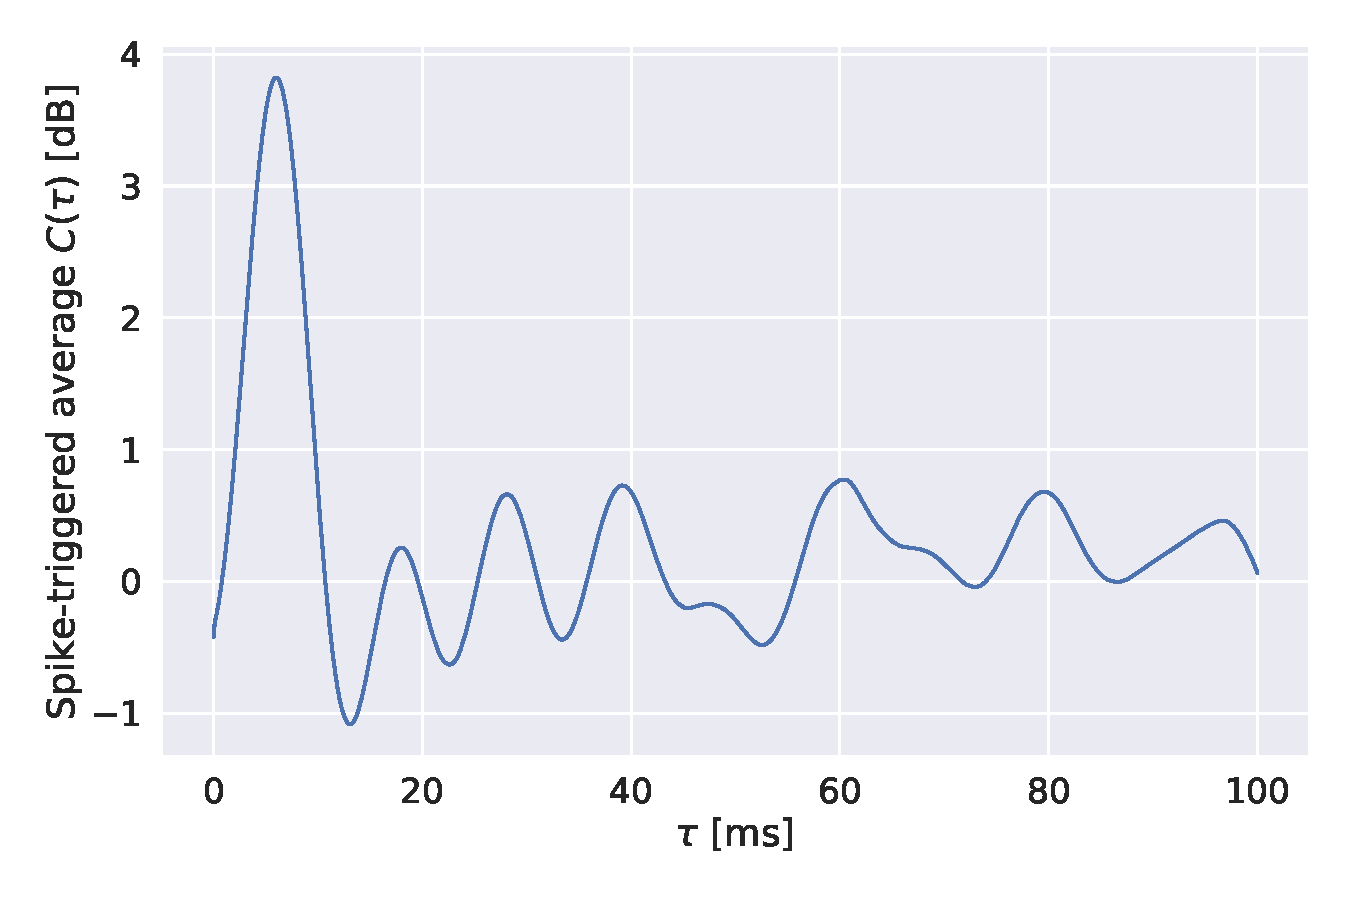
\includegraphics[width=0.8\textwidth]{4_filtro.pdf}
    \caption{\textit{spike-triggered average} $C(\tau)$ del estimulo en función de tiempo $\tau$.}
    \label{04:fig:filtro}
\end{figure}

% Otra razón por la cual la cantidad hSiST A (τ ) es de interés es que, si aproximamos al estı́mulo por ruido blanco, resulta que hSiST A (τ ) es proporcional al filtro que da la mejor predicción lineal de la tasa de disparo asociada a la neurona.

% Esta función corresponde al término lineal en la expansión de Volterra en caso de despreciar la autocorrelación del estı́mulo, suponer que el estı́mulo tiene valor medio cero y suponer que el estı́mulo es estacionario.